\section{逐层机制分析}

\subsection{为什么要做 Layer-wise Analysis}

前面的分析回答了“推理沿哪个扩散轴展开”，但还没有回答“在单个 diffusion step 内，DiT 各层分别做什么”。因此论文进一步分析 Transformer 层内部 hidden states，试图识别不同层的功能分工。

这一节有两个互补方法：token-level visualization 用来观察每层激活分布，latent swapping 用来测试某一层表示是否对最终推理结果具有因果影响。

\subsection{Forward Hook 与中间表示捕获}

在 PyTorch 中，forward hook 是一种监听机制：在某一层前向计算完成时，额外保存该层输出。中间表示当然在计算过程中存在，但默认不会保留下来供分析；如果不注册 hook，推理结束后通常只能拿到最终输出。

论文在 Wan2.2-I2V-A14B 的 DiT 各层注册 forward hook，捕获每层 hidden state。作者特别提取 positive CFG pass 的隐藏状态，以隔离带 prompt 条件的主要推理路径，而不是把有条件、无条件和 guidance 混合后的表示混在一起分析。

\subsection{Token 序列与时空网格}

视频 latent 自然可以写成 5 维结构，但 Transformer 内部通常把时空 patch 展平成 token 序列。论文捕获到的原始 hidden state 形式是

\begin{equation}
    \mathrm{feat} \in \mathbb{R}^{B \times N \times D},
\end{equation}

其中 $N$ 是 token 总数，$D$ 是 embedding 维度，原始笔记中记录 $D=5120$。这里的“原始特征”不是原始像素，而是 hook 直接截获的、尚未恢复时空结构的内部 token 表示。

由于每个 token 原本对应一个时空 patch，可根据 patch embedding 记录的网格尺寸 $(f,h,w)$ reshape 回

\begin{equation}
    (B,f,h,w,D),
\end{equation}

其中 $f$ 是时间格子数，$h,w$ 是空间格子数。

\subsection{Activation Energy}

每个时空位置上的 token 是一个 $D$ 维向量：

\begin{equation}
    u_{f,h,w} \in \mathbb{R}^{D}.
\end{equation}

为了画热力图，需要把高维向量压成一个标量。论文在通道维度上计算 L2 范数：

\begin{equation}
    \|u_{f,h,w}\|_2
    = \sqrt{\sum_{d=1}^{D} u_{f,h,w,d}^{2}}.
\end{equation}

这个值被用作 activation intensity 或 energy，表示该 patch 在当前层中的整体表征幅值。它不是严格因果重要性证明，而是可视化 proxy：范数大通常说明该位置的隐藏表示更活跃、更多通道响应明显，更可能是模型当前正在强烈编码的区域。

从线性代数角度看，若后续层有线性映射 $W$，则

\begin{equation}
    \|Wu\| \le \|W\|\|u\|,
\end{equation}

所以较大范数意味着潜在输出影响上界更大。但这只是解释性依据，不等于“范数大必然决定答案”。因此论文还需要 latent swapping 提供更强的因果证据。

\subsection{Figure 6(a)：层功能分工}

Figure~\ref{fig:figure6} 展示了不同 DiT layers 的 token activation heatmap。每一行对应不同 DiT 层，每一列对应视频帧或示例中的帧。亮区表示该 patch 的 hidden vector L2 norm 较大。

\begin{figure}[H]
    \centering
    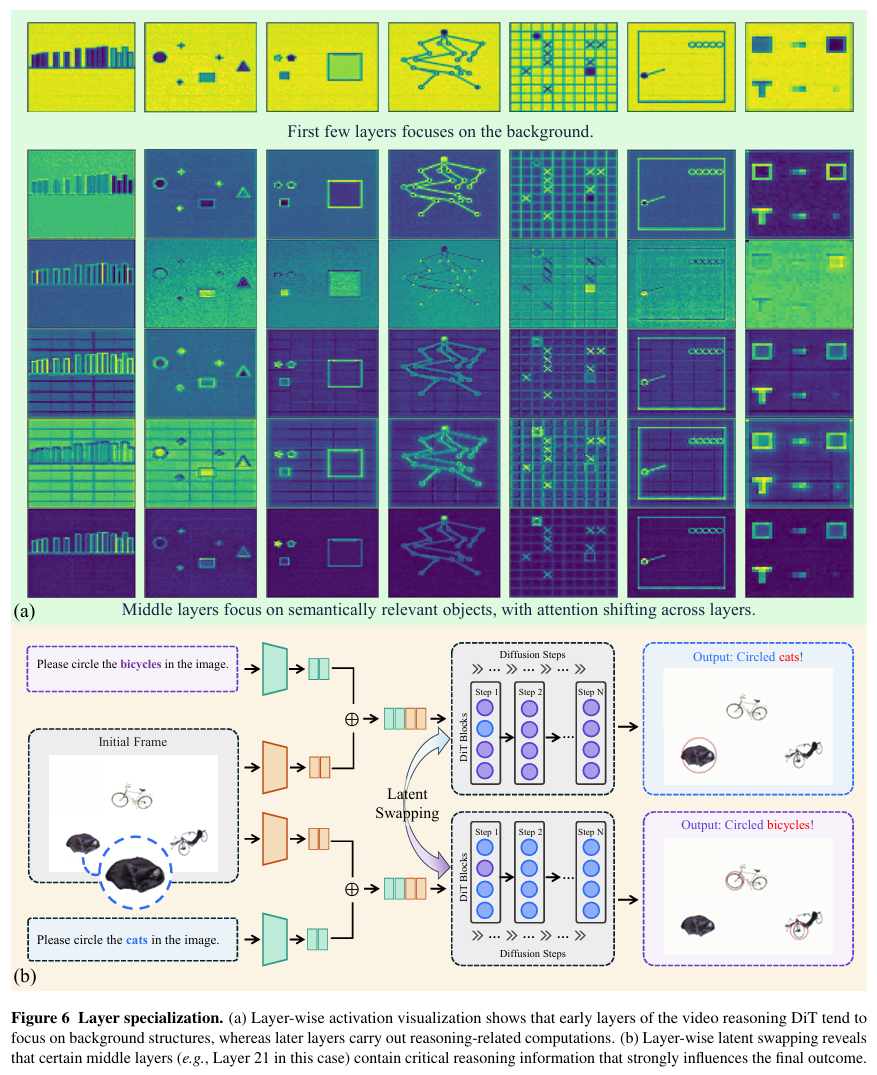
\includegraphics[width=0.96\textwidth]{figures/figure6.png}
    \caption{逐层 token 级可视化与 latent swapping：DiT 层内部存在从感知到推理的功能分工。}
    \label{fig:figure6}
\end{figure}

主要观察如下：

\begin{itemize}
    \item 浅层通常关注背景、场景边界、全局轮廓和基本几何结构。
    \item 中层开始把激活集中到前景对象、prompt 指定对象和语义相关区域。
    \item 更深层进一步整合任务相关结构，形成与运动、交互和最终决策有关的表示。
\end{itemize}

这说明在单个 diffusion step 内，模型也不是所有层都做同一件事，而是存在层级处理结构：早层做 dense perceptual understanding，中层做对象级聚焦和推理，后层整合 latent 状态，准备交给下一个 diffusion step。

\subsection{Latent Swapping 的因果意义}

Token energy heatmap 只能说明相关性，不能证明某一层决定答案。为此论文做逐层 latent swapping：构造两个不同对象配置，在某一层 $k$ 将原样本 hidden state 替换为另一样本的 hidden state：

\begin{equation}
    \tilde{U}^{(k)} \leftarrow U_{\mathrm{alt}}^{(k)},
\end{equation}

其他层保持原始路径。若替换某层后最终识别结果翻转，说明该层表示对最终决策有直接影响。

论文观察到，中后层，尤其是约第 20 层附近的表示替换，会导致目标识别或定位结果翻转。这提供了因果证据：中间到后期层确实编码了决定性语义信息，而不只是被热力图“看起来更亮”。

\subsection{Diffusion Step 与 DiT Layer 的区别}

阅读这篇论文时必须分清两个轴：

\begin{itemize}
    \item diffusion step：采样过程中的时间步，例如从噪声到干净 latent 的第 1 步、第 20 步、第 50 步。
    \item DiT layer：在某一个 diffusion step 内，latent 经过的 Transformer block 深度，例如 Layer 0 到 Layer 39。
\end{itemize}

CoS 分析关注 step 轴，说明推理沿去噪过程展开。Layer-wise analysis 关注 layer 轴，说明每个 step 内部还有从感知到推理的层级分工。二者叠加起来，才构成本文对视频推理机制的完整解释。
